\documentclass{standalone}
\usepackage{tikz}


\begin{document}

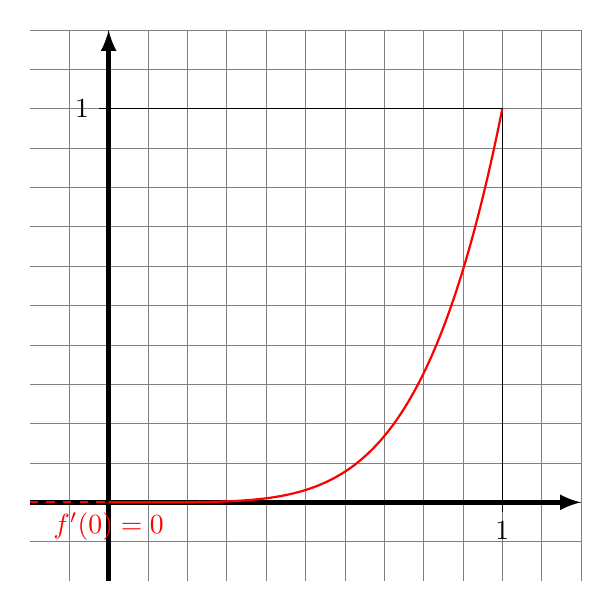
\begin{tikzpicture}[scale=5,axis/.style={-latex,ultra thick},graph/.style={red,thick}]
  \draw[help lines] (-0.2,-0.2) grid[step=0.1cm] (1.2,1.2);
  \draw (0,0) rectangle (1,1);
  \draw[axis] (-0.2,0) -- (1.2,0);
  \draw[axis] (0,-0.2) -- (0,1.2);
  \draw (-0.025,1) -- (0,1) node[left,at start] {$1$};
  \draw (1,0) -- (1,-0.025) node[below] {$1$};
  
  \draw[graph] plot[domain=0:1,smooth,samples=1000] (\x,{\x^5});
  \draw[red,thick,dashed] (-0.2,0) -- (0.2,0) node[below,midway] {$f'(0) = 0$};
\end{tikzpicture}

\end{document}